For detecting if a new state has occurred a method for detecting this has to be developed. The method will consist of two steps:

\begin{enumerate}
	\item Detect if human interaction has occurred.
	\item If human interaction occured, then detect if ball position or number of ball changed.
\end{enumerate}


\subsection{Detect human interaction:}
The first step is to detect weather or not the cloth is occluded. This occlusion could be caused by human interaction or foreign object placed within the cloth of the table. Detection will be used before finding position of balls. If the table is detected to be occluded then there will be no detection of balls before the table is interacted with. This will bring down faulty detections caused by cue or foreign objects.\\

When the table is detected, as described in section \ref{sec:table-locate}, a mask for the cloth is made. This mask is made from a contour which has many different properties such as area and perimeter. These properties can be used when identifying if occlusions are present. By comparing the current image mask together with the mask made in the calibration and finding the difference in area or perimeter, detection should be possible.\\

For this purpose of this method only foreign object introduced from the edge and in will be considered as a foreign object. Therefore a que from the edge of the table would be detected, but a ball or laying on the table will not.

Occlusion area factor:
\begin{equation}
\lambda = \frac{A_{current}}{A_{calibrated}}
\label{eq:area}
\end{equation}

Occlusion perimeter factor:
\begin{equation}
\kappa = \frac{P_{current}}{P_{calibrated}}
\label{eq:perimeter}
\end{equation}

\textbf{Test image with values and factors:}\\
\begin{tabular}{|l|c|c|l|l|c|}
\hline - & Image & Mask & A \& $\lambda$ & P \& $\kappa$ & Occlusion \\ 
\hline

\multirow{2}{*}{Calibrated.} & \multirow{2}{*}{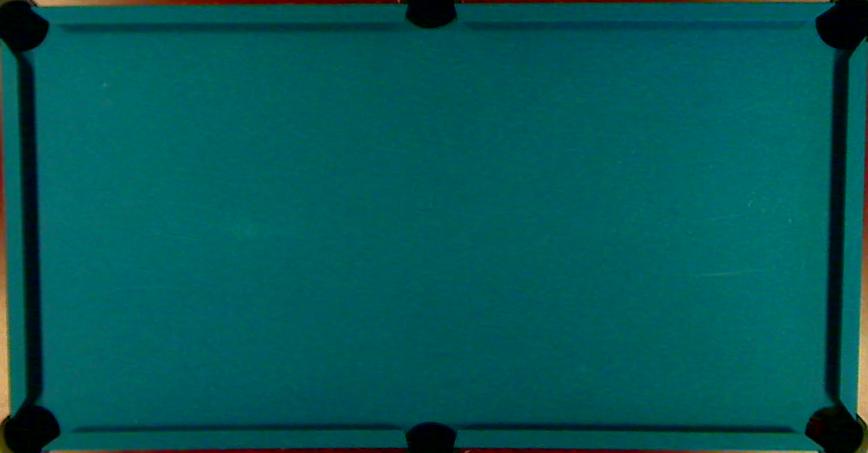
\includegraphics[scale=0.05]{../images/1/calibimg.png}} & \multirow{2}{*}{
\includegraphics[scale=0.05]{../images/1/calibmask.png}} & A = 369861 &  & \multirow{2}{*}{}\\  
& & & & P = 3153 & \\
\hline

\multirow{2}{*}{Empty table.} & \multirow{2}{*}{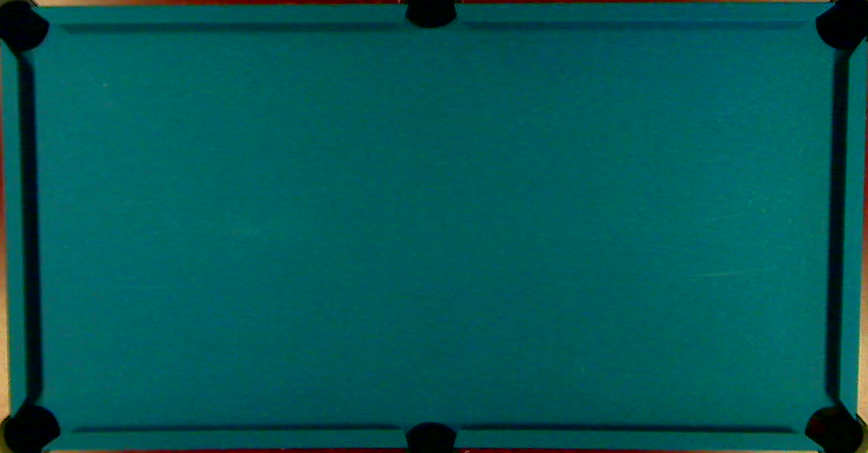
\includegraphics[scale=0.05]{../images/1/0_img.png}} & \multirow{2}{*}{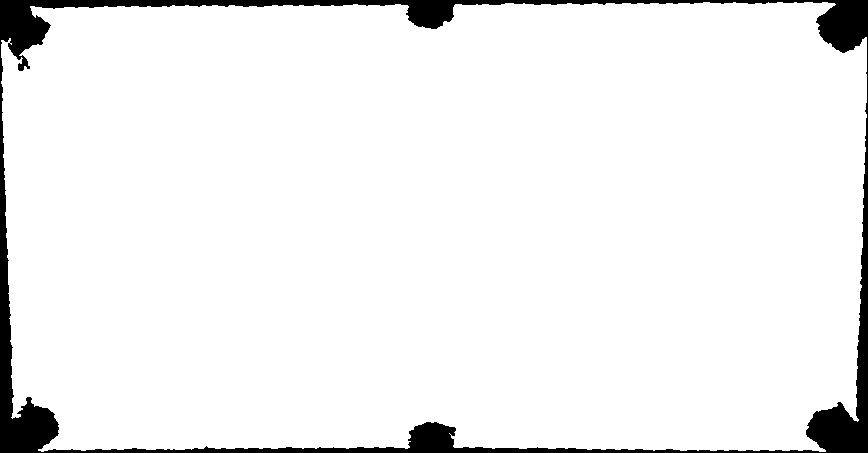
\includegraphics[scale=0.05]{../images/1/0_mask.png}} & A = 369518 & P = 3185 & \multirow{2}{*}{}\\  
& & & $\lambda$ = 0.9991 & $\kappa$ = 1.0099 & \\
\hline

\multirow{2}{*}{With balls.} & \multirow{2}{*}{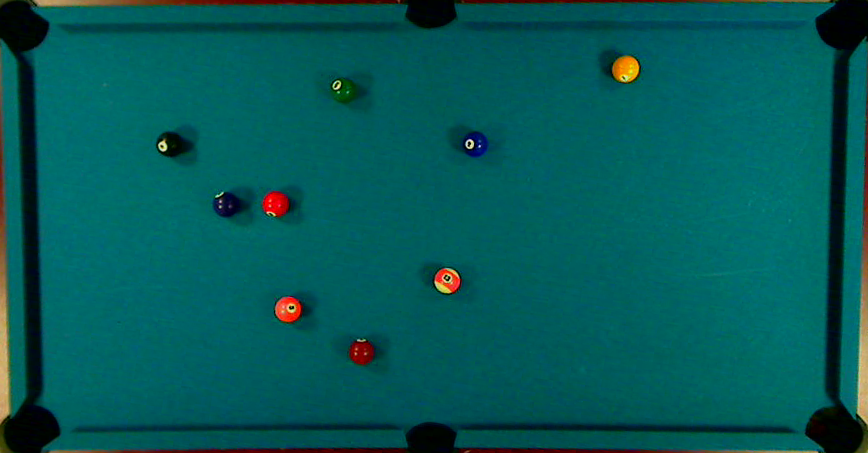
\includegraphics[scale=0.05]{../images/1/1_img.png}} & \multirow{2}{*}{
\includegraphics[scale=0.05]{../images/1/1_mask.png}} & A = 369852 & P = 3193 & \multirow{2}{*}{}\\ 
& & & $\lambda$ = 1 & $\kappa$ = 1.0127 & \\
\hline

\multirow{2}{*}{With person.} & \multirow{2}{*}{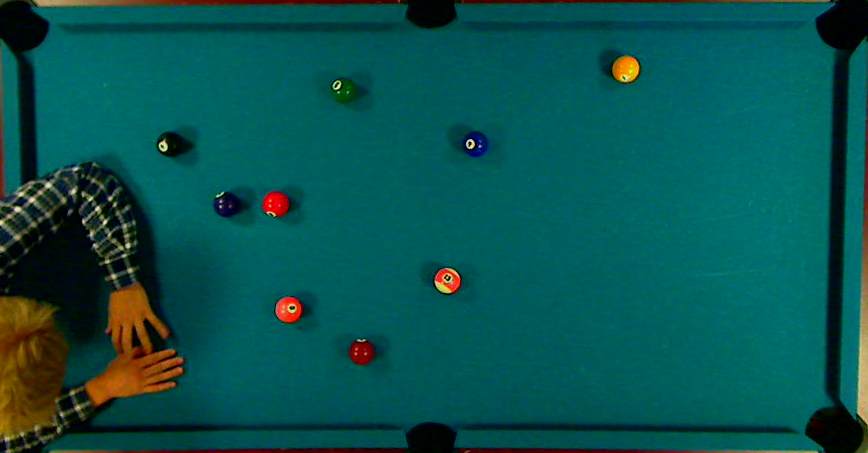
\includegraphics[scale=0.05]{../images/1/2_img.png}} & \multirow{2}{*}{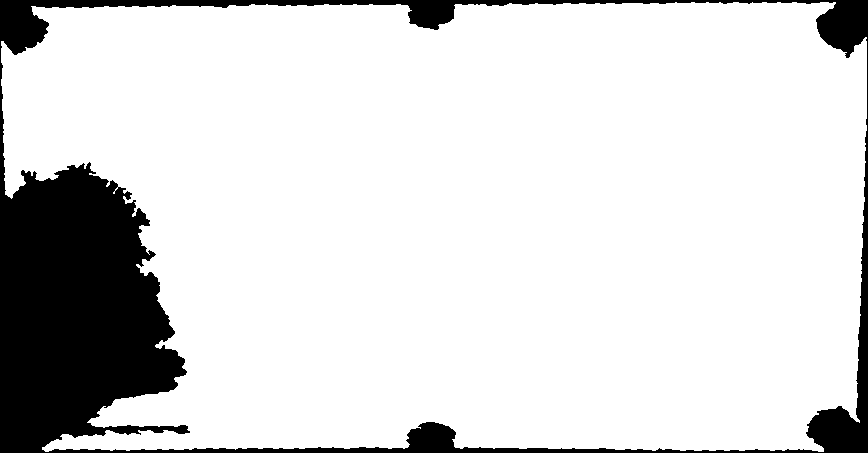
\includegraphics[scale=0.05]{../images/1/2_mask.png}} & A = 334652 & P = 3866 & \multirow{2}{*}{\checkmark}\\  
& & & $\lambda$ = 0.9048 & $\kappa$ = 1.2258 & \\
\hline

\multirow{2}{*}{Que on table I.} & \multirow{2}{*}{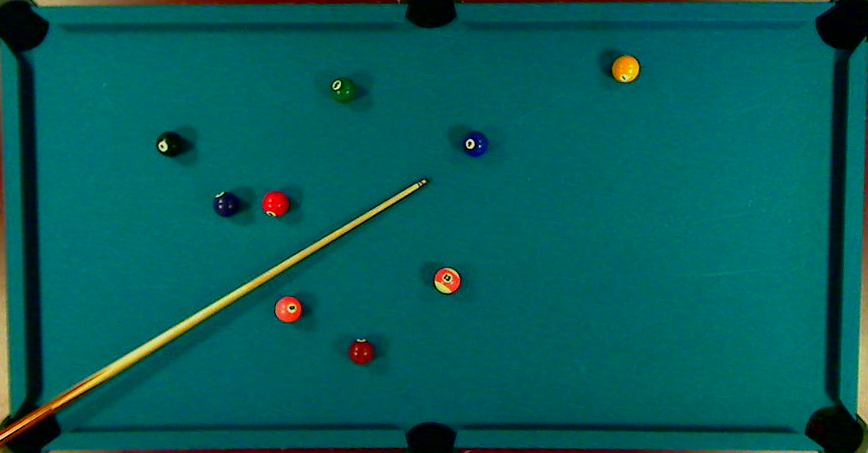
\includegraphics[scale=0.05]{../images/1/3_img.png}} & \multirow{2}{*}{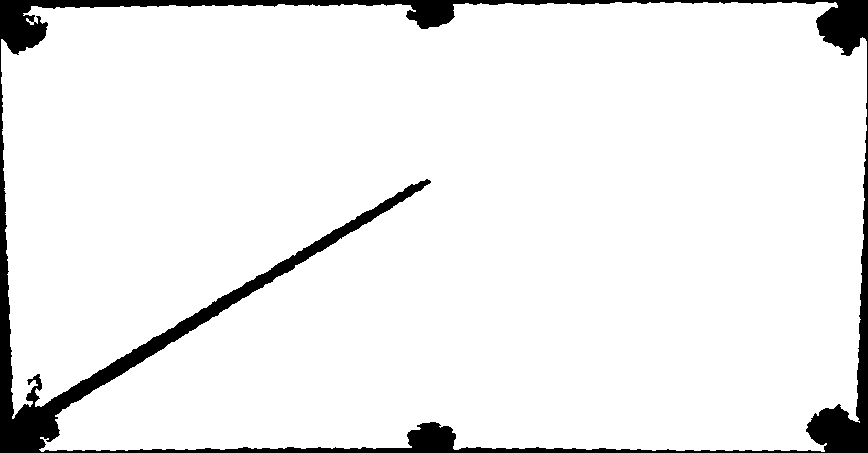
\includegraphics[scale=0.05]{../images/1/3_mask.png}} & A = 364515 & P = 4287 & \multirow{2}{*}{\checkmark}\\  
& & & $\lambda$ = 0.9855 & $\kappa$ = 1.3594 & \\
\hline

\multirow{2}{*}{Que on table II.} & \multirow{2}{*}{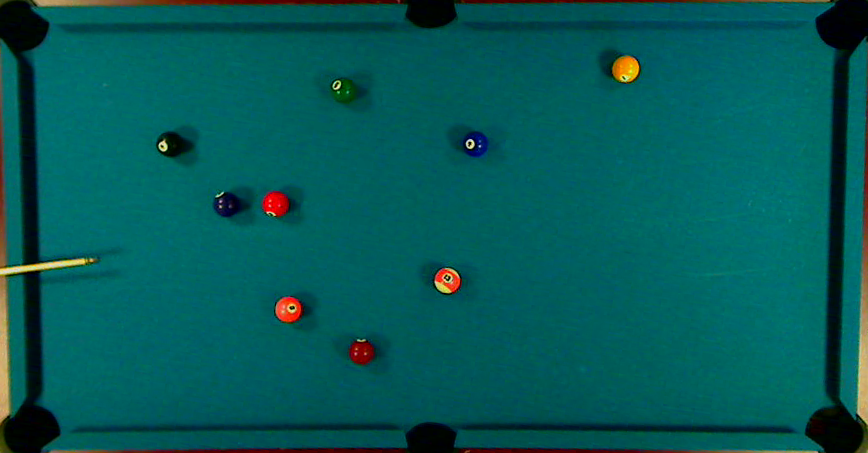
\includegraphics[scale=0.05]{../images/1/4_img.png}} & \multirow{2}{*}{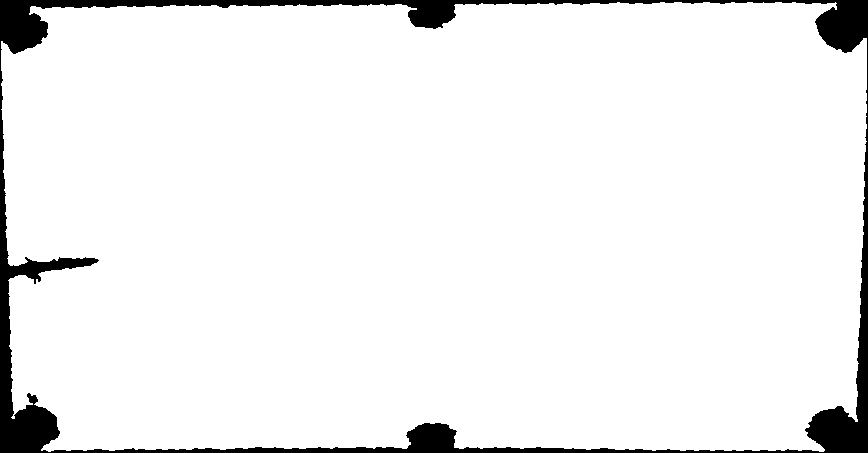
\includegraphics[scale=0.05]{../images/1/4_mask.png}} & A = 368846 & P = 3324 & \multirow{2}{*}{\checkmark}\\  
& & & $\lambda$ = 0.9973 & $\kappa$ = 1.0541 & \\
\hline

\multirow{2}{*}{Que on table III.} & \multirow{2}{*}{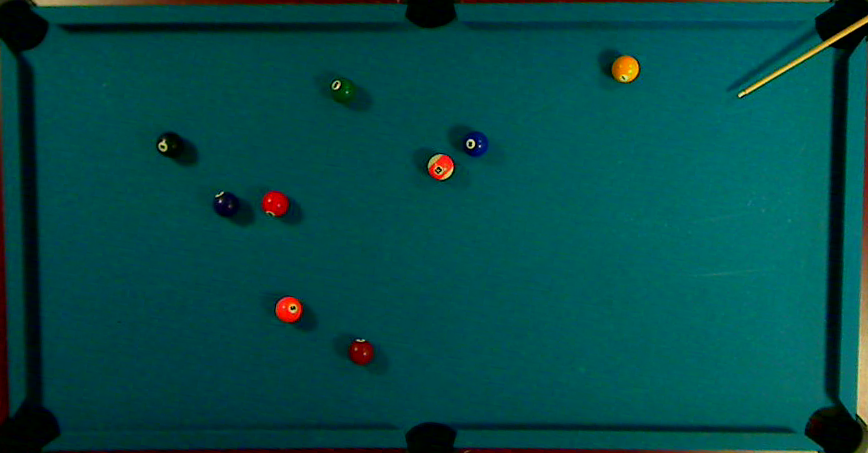
\includegraphics[scale=0.05]{../images/1/11_img.png}} & \multirow{2}{*}{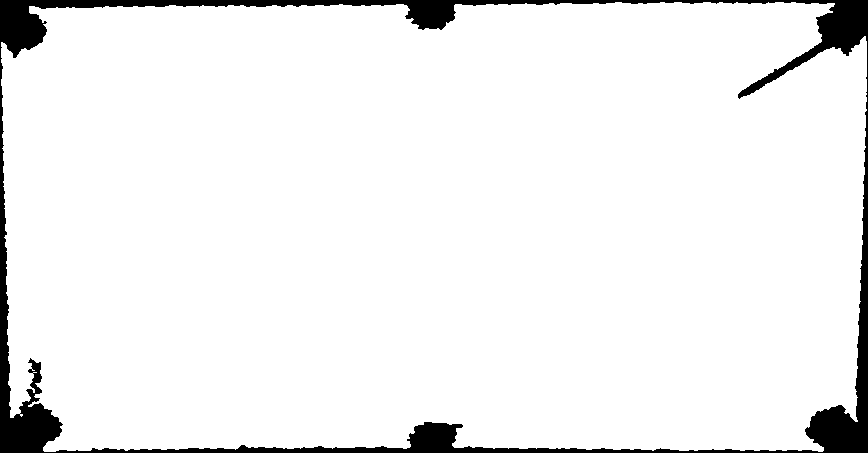
\includegraphics[scale=0.05]{../images/1/11_mask.png}} & A = 368555 & P = 3566 & \multirow{2}{*}{\checkmark}\\ 
& & & $\lambda$ = 0.9965 & $\kappa$ = 1.1307 & \\
\hline

\multirow{2}{*}{Que on table IV.} & \multirow{2}{*}{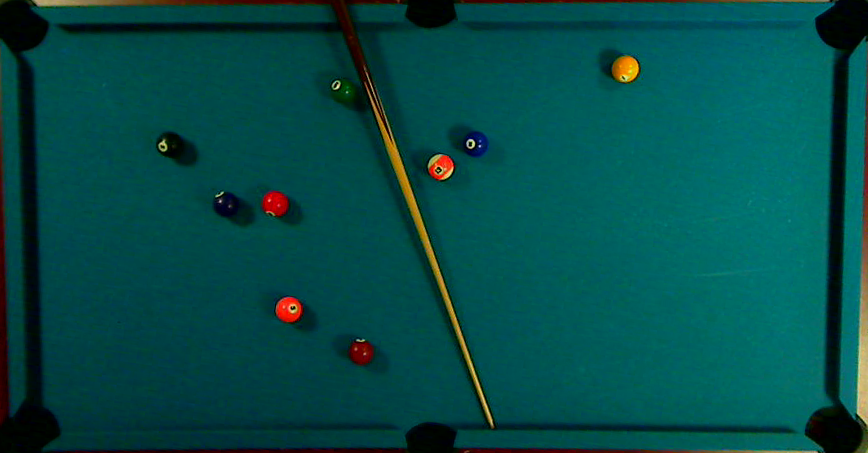
\includegraphics[scale=0.05]{../images/1/12_img.png}} & \multirow{2}{*}{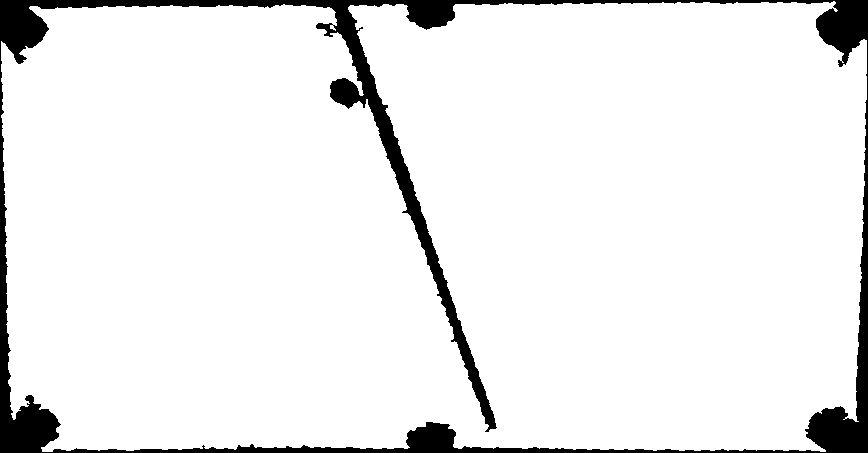
\includegraphics[scale=0.05]{../images/1/12_mask.png}} & A = 362749 & P = 4458 & \multirow{2}{*}{\checkmark}\\ 
& & & $\lambda$ = 0.9808 & $\kappa$ = 1.4138 & \\
\hline

\multirow{2}{*}{Chair on table.} & \multirow{2}{*}{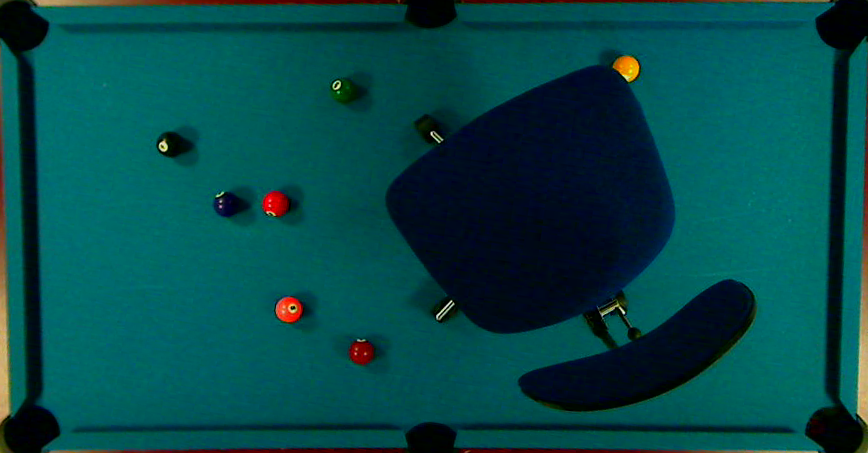
\includegraphics[scale=0.05]{../images/1/5_img.png}} & \multirow{2}{*}{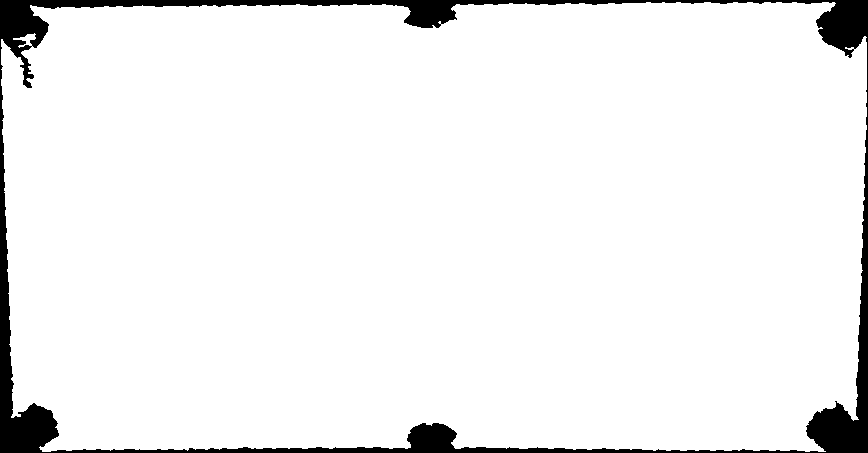
\includegraphics[scale=0.05]{../images/1/5_mask.png}} & A = 369881 & P = 3336 & \multirow{2}{*}{}\\  
& & & $\lambda$ = 1 & $\kappa$ = 1.0578 & \\
\hline

\multirow{2}{*}{Shadow.} & \multirow{2}{*}{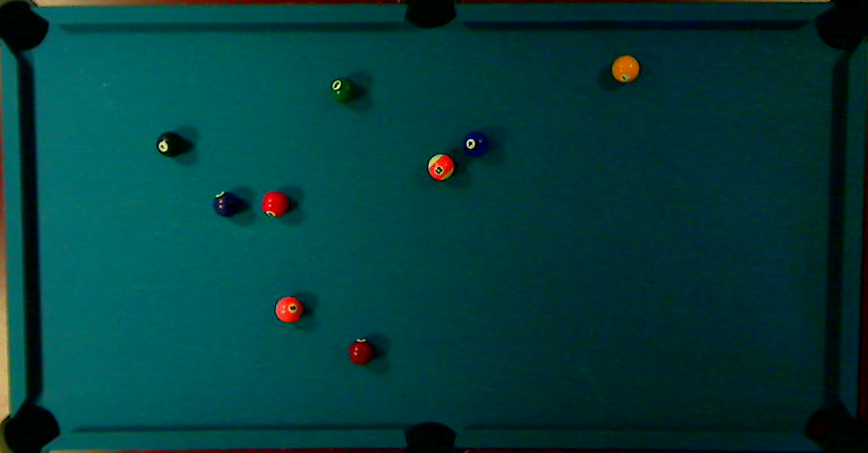
\includegraphics[scale=0.05]{../images/1/6_img.png}} & \multirow{2}{*}{
\includegraphics[scale=0.05]{../images/1/6_mask.png}} & A = 366844 & P = 3780 & \multirow{2}{*}{}\\ 
& & & $\lambda$ = 0.9918 & $\kappa$ = 1.1986 & \\
\hline

\multirow{2}{*}{Lighting I.} & \multirow{2}{*}{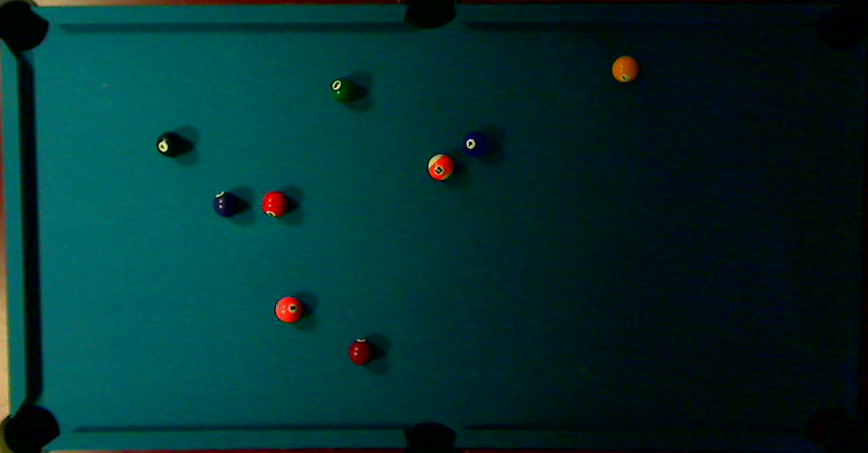
\includegraphics[scale=0.05]{../images/1/7_img.png}} & \multirow{2}{*}{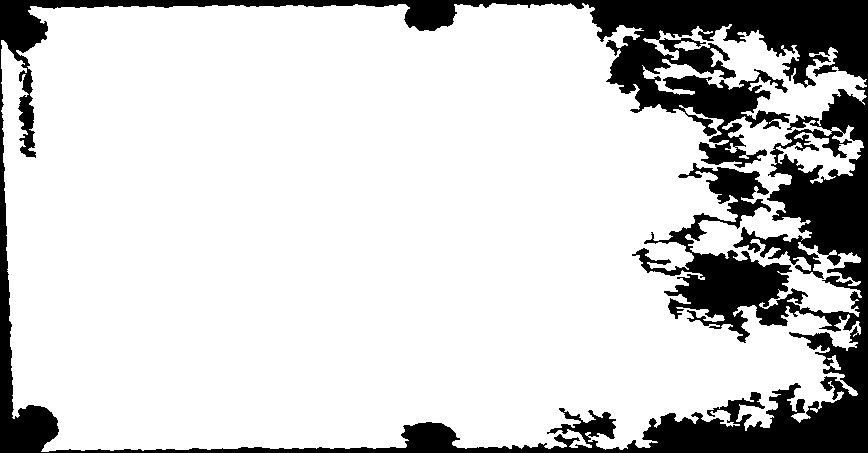
\includegraphics[scale=0.05]{../images/1/7_mask.png}} & A = 314105 & P = 12473 & \multirow{2}{*}{}\\ 
& & & $\lambda$ = 0.8493 & $\kappa$ = 3.9550 & \\
\hline

\multirow{2}{*}{Lighting II.} & \multirow{2}{*}{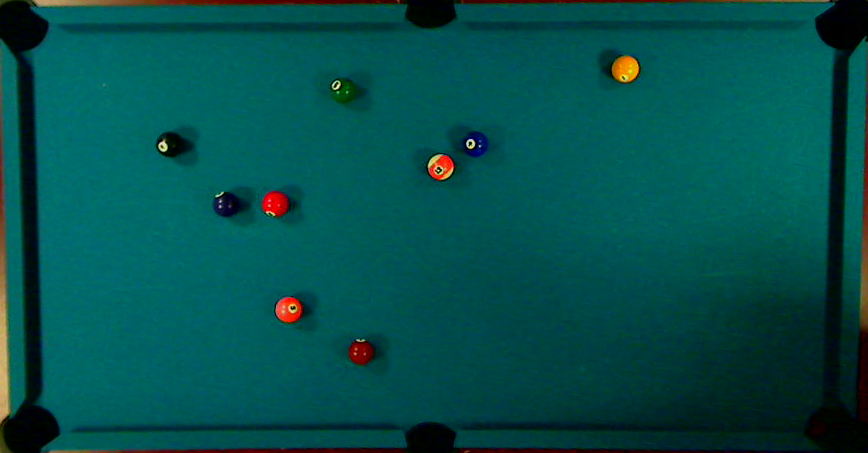
\includegraphics[scale=0.05]{../images/1/8_img.png}} & \multirow{2}{*}{
\includegraphics[scale=0.05]{../images/1/8_mask.png}} & A = 368666 & P = 3339 & \multirow{2}{*}{}\\ 
& & & $\lambda$ = 0.9968 & $\kappa$ = 1.0589 & \\
\hline

\multirow{2}{*}{Lighting III.} & \multirow{2}{*}{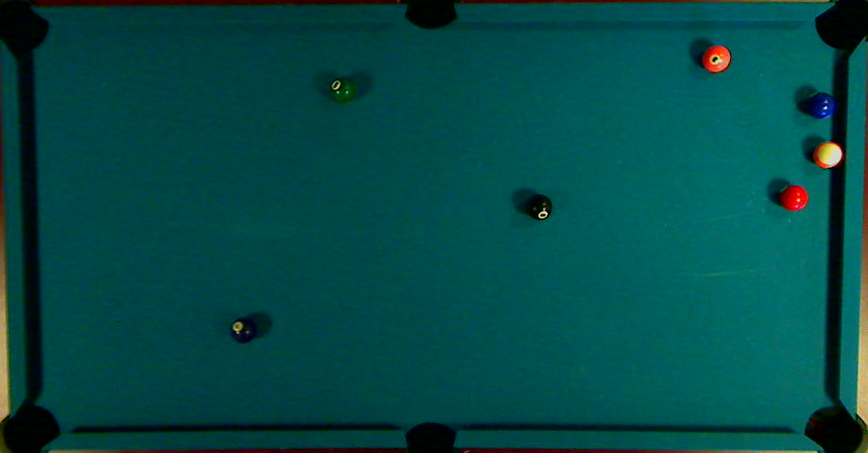
\includegraphics[scale=0.05]{../images/1/14_img.png}} & \multirow{2}{*}{
\includegraphics[scale=0.05]{../images/1/14_mask.png}} & A = 368783 & P = 3291 & \multirow{2}{*}{}\\ 
& & & $\lambda$ = 0.9971 & $\kappa$ = 1.0436 & \\
\hline

\multirow{2}{*}{Lighting IV.} & \multirow{2}{*}{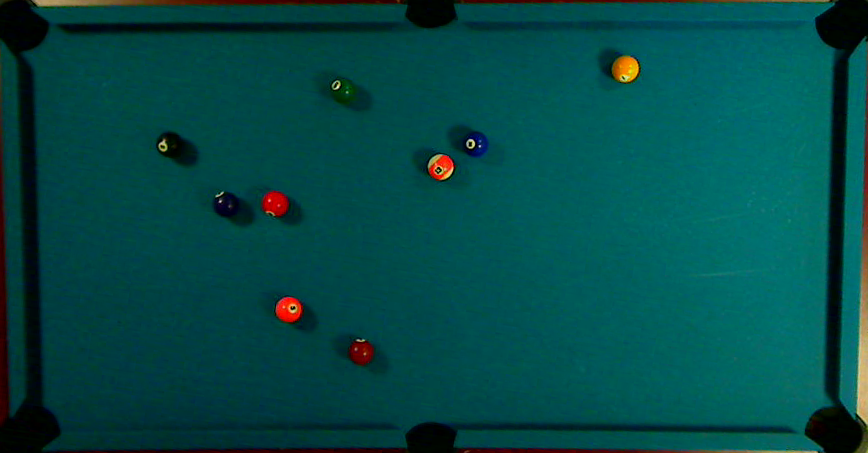
\includegraphics[scale=0.05]{../images/1/9_img.png}} & \multirow{2}{*}{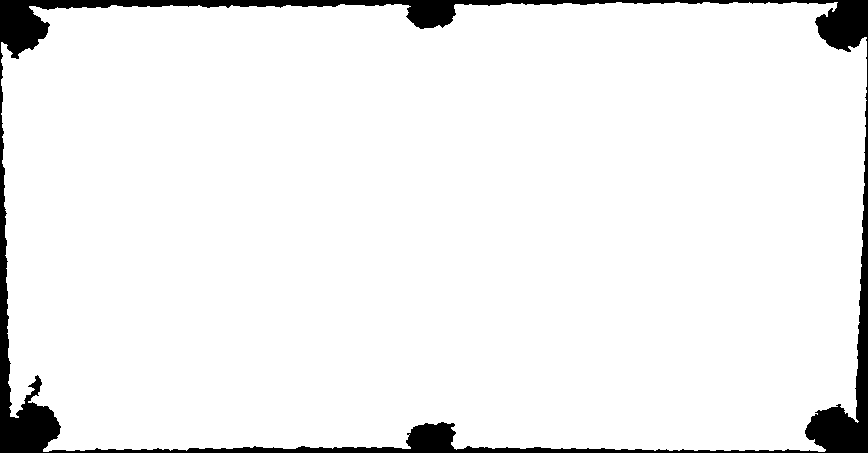
\includegraphics[scale=0.05]{../images/1/9_mask.png}} & A = 369481 & P = 3249 & \multirow{2}{*}{}\\ 
& & & $\lambda$ = 0.9990 & $\kappa$ = 1.0305 & \\
\hline

\multirow{2}{*}{With ladder.} & \multirow{2}{*}{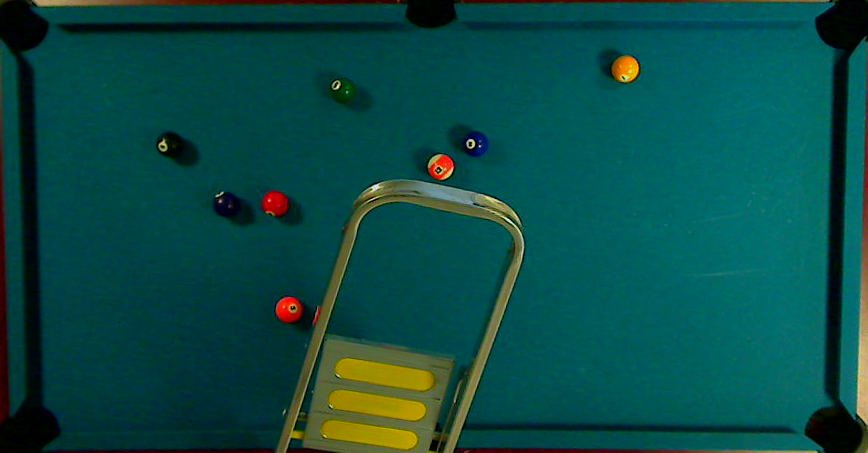
\includegraphics[scale=0.05]{../images/1/10_img.png}} & \multirow{2}{*}{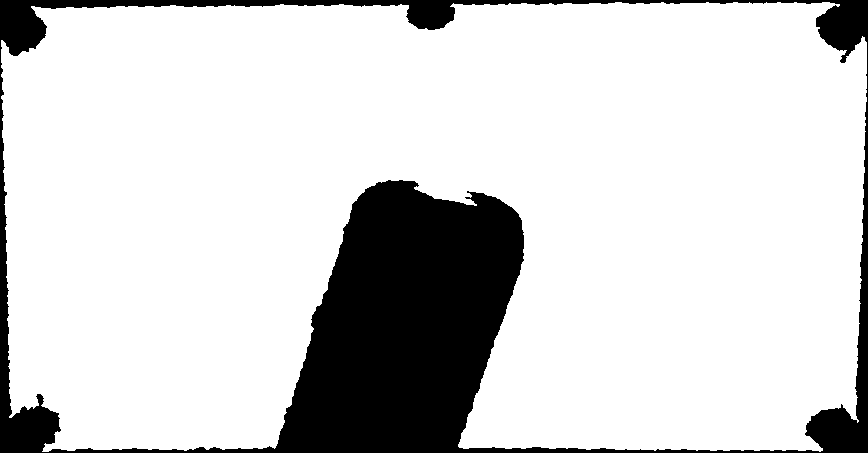
\includegraphics[scale=0.05]{../images/1/10_mask.png}} & A = 324054 & P = 3721 & \multirow{2}{*}{\checkmark}\\ 
& & & $\lambda$ = 0.8762 & $\kappa$ = 1.1801 & \\
\hline

\multirow{2}{*}{Triangle on table.} & \multirow{2}{*}{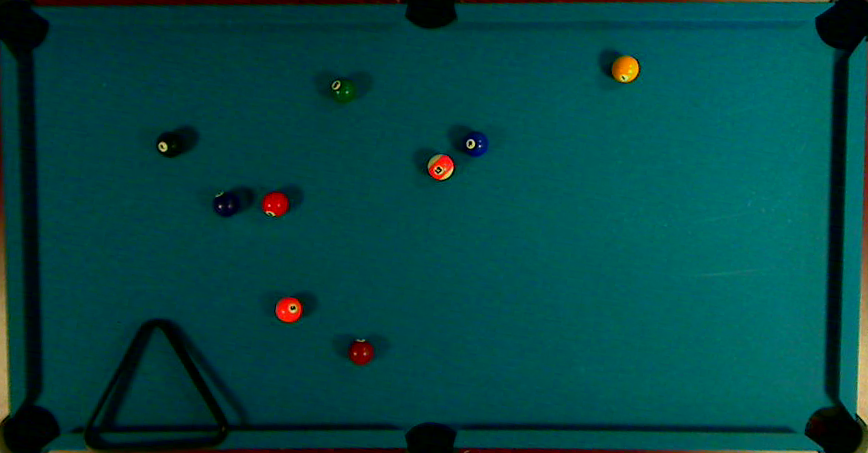
\includegraphics[scale=0.05]{../images/1/13_img.png}} & \multirow{2}{*}{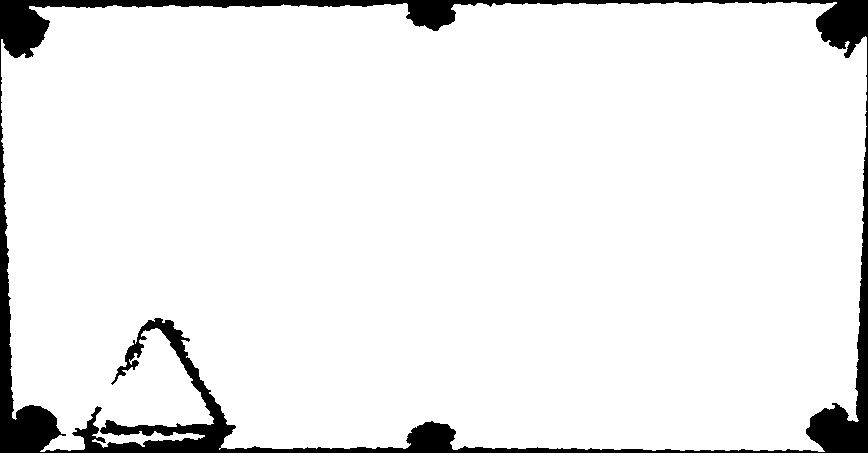
\includegraphics[scale=0.05]{../images/1/13_mask.png}} & A = 364360 & P = 4243 & \multirow{2}{*}{\checkmark}\\ 
& & & $\lambda$ = 0.9851 & $\kappa$ = 1.3456 & \\
\hline

\multirow{2}{*}{Hand on table.} & \multirow{2}{*}{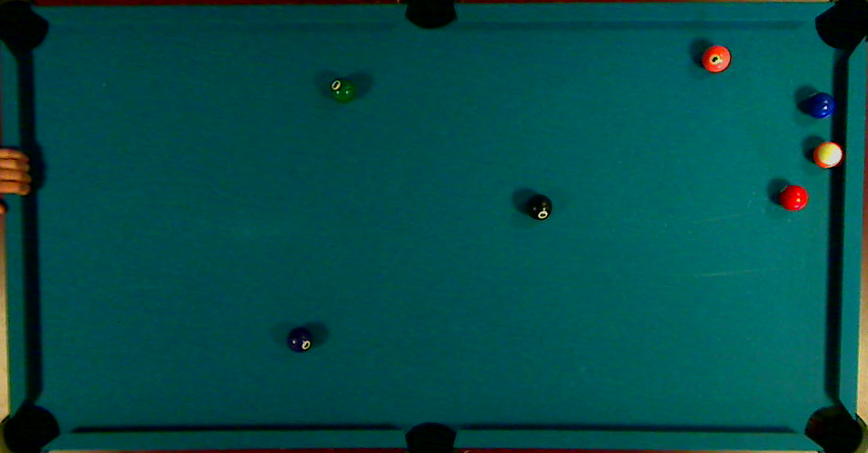
\includegraphics[scale=0.05]{../images/1/15_img.png}} & \multirow{2}{*}{
\includegraphics[scale=0.05]{../images/1/15_mask.png}} & A = 364787 & P = 3895 & \multirow{2}{*}{\checkmark}\\ 
& & & $\lambda$ = 0.9863 & $\kappa$ = 1.2351 & \\
\hline

\end{tabular} 

\textbf{Plot of factors:}\\
The plot\ref{fig:occlusion_plot} does not contain "Lighting I" factors since the perimeter is very high compared to the normal. This is due to the light being altered too much which is not allowed as written in the requirement specification in section \ref{sec:reqspec}.

\begin{figure}[H]
\begin{center}
\leavevmode
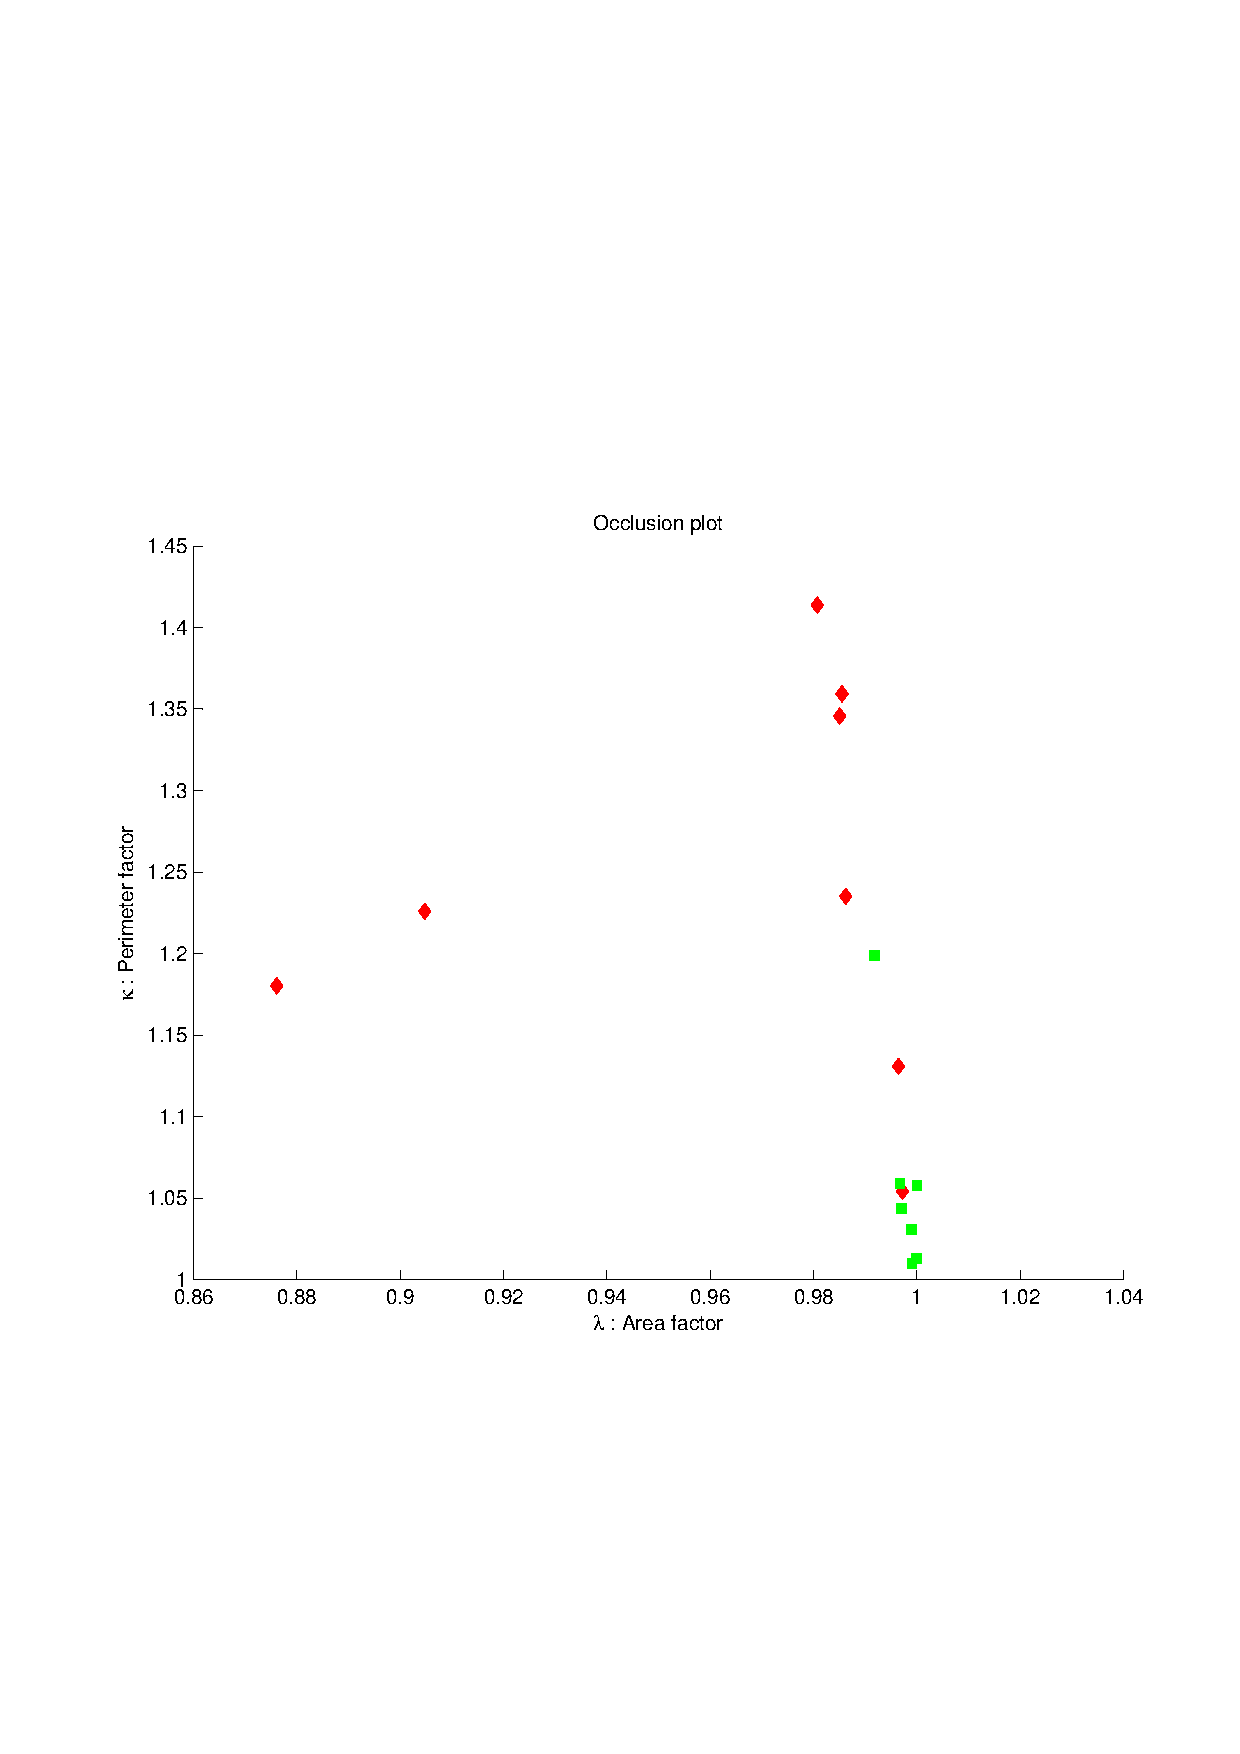
\includegraphics[width=0.7\textwidth]{images/occlusion_plot}
\end{center}
\caption{Occlusion plot. Red triangles are occlusions and green squares are not.}
\label{fig:occlusion_plot}
\end{figure}

The red triangle (occlusion) that lie within the green square (non occlusion) is "Que on table II" which is occlusion by a small part of the que.\\

The green square (non occlusion) that lie between two red diamonds (occlusions) is "Shadow" where a shadow is introduced by a person. This was done while also changing the light. The area factor is very close to normal, but the perimeter is not due to significant light changes underneath the left cushion.\\

The following mean-values have been calculated for the non occlusions:\\

$\mu_{\lambda} = 0.99$\\
$\mu_{\kappa} = 1.06$\\

The occlusion detection is only done to determine if the balls position should be re-evaluated. Therefore it is not crucial that the detection is 100\% correct. A wrong detection will simply cause a re-evaluation of the balls position which would show no movement. Therefore it is optimal to make a "paranoid" classifier that would be more inclined to assume a occlusion than not.\\

Since an introduction of a foreign object will always make the contour area smaller and the perimeter bigger the values for a detection will be set to:

\begin{center}
$\lambda_{detection} if \lambda < 0.99$ \\
or\\
$\kappa_{detection} if \kappa > 1.04$.
\end{center}

Instead of a decision tree, a linear discriminant function could have been made. The outcome is roughly the same and for simplification a decision tree was chosen.

\subsection{Detect movement and number of balls:}
After an human interaction it is required to detect if movement of the balls or change in number of ball is present. If this is the case the positions of the balls are saved as a new state. If it is not the case the system will wait for the next human interaction.

To detect if movement or number has changed the current number of balls and their positions will be compared to the last state.

